\documentclass[a4paper,11.5pt]{article}
\usepackage[latin1]{inputenc}
\usepackage[T1]{fontenc}
\usepackage[english]{babel}
\usepackage{graphicx}
\usepackage{amsmath}
\usepackage{amsfonts}
\usepackage{multirow}
\usepackage{booktabs}
\usepackage{bbold}
\usepackage{mathtools}
\usepackage{mathrsfs}
\usepackage{enumitem}
\usepackage{array}

\setlength{\parindent}{0pt}
\DeclarePairedDelimiter{\floor}{\lfloor}{\rfloor}
\DeclarePairedDelimiter{\ceil}{\lceil}{\rceil}

\newcommand{\vt}{\boldsymbol}

\title{Digital Communications - HW3}
\author{Jacopo Pegoraro, Edoardo Vanin}
\date{21/05/2018}

\begin{document}

\maketitle

\section*{Problem}

We have to implement six different versions of the receiver structure in a QPSK modulation scheme. First we present the setup of the transmitter and the channel as given, the we analyze the different configurations one by one and give a brief discussions of the resulting probabilities of symbol error obtained from simulation over different values of the SNR at the channel output, $\Gamma$. 

\section*{Transmitter and Channel}

The system takes a sequence of input symbols $a_k$ at sampling time $T=1$ and applies an upsampling of factor 4, obtaining $a_k'$ at $T/4$. This new sequence is then filtered by $q_c$ as described by the following difference equation:
\begin{equation}
s_c(nT/4) = 0.67 s_c((n-1)T/4) + 0.7424 a_{n-5}
\end{equation}
After the filtering white noise is added. The SNR at the channel output for all the configurations in this first phase is $\Gamma = 10$ dB, so from the following relations we can derive $\sigma_w^2$, the variance of the complex valued Gaussian noise:
\begin{equation}
\Gamma = \frac{M_{s_c}}{N_0\frac{1}{T}} = \frac{\sigma_a^2 E_{q_c}}{\sigma_w^2} \longrightarrow \sigma_w^2 = \frac{\sigma_a^2 E_{q_c}}{\Gamma} = 2\sigma_I^2
\end{equation}
where $\sigma_I^2$ is the variance per component. In addition we can also compute the PSD as $N_0=\sigma_w^2 T_c=\sigma_w^2/4$, because the sampling time $T_c$ at which we add the noise is $T/4$.
In figure \ref{fig:qc} we plot the impulse response and the frequency response of the filter $q_c$.
This implementation of the transmitter is the same for all the following discussion.

\begin{figure}[ht]
	\begin{center}   
		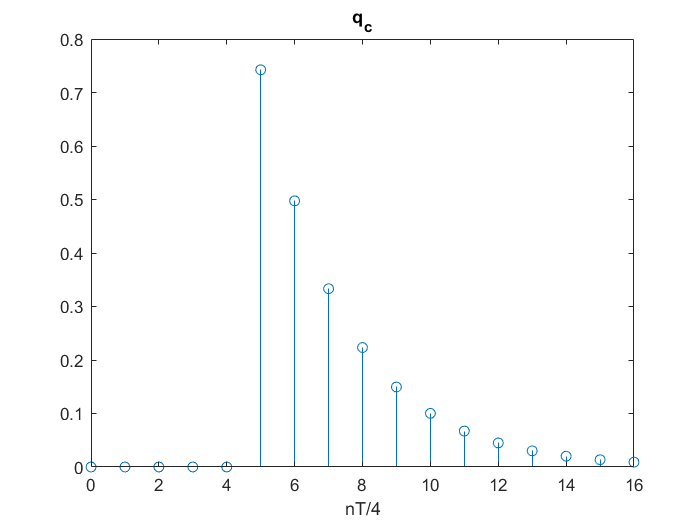
\includegraphics[width=\textwidth]{figs/q_c.png} 
		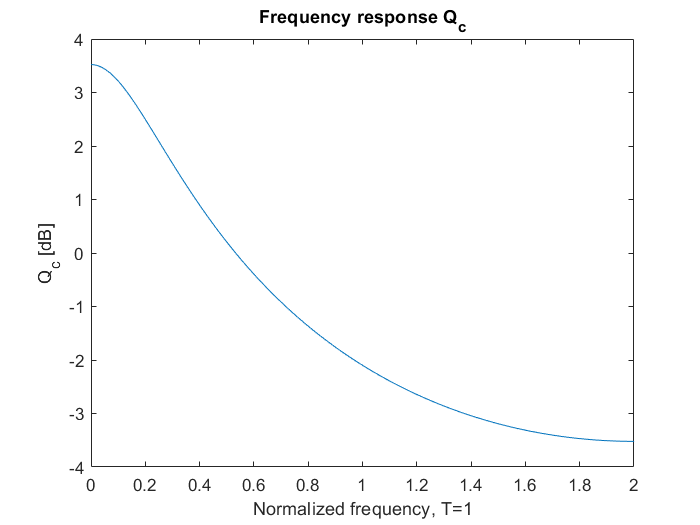
\includegraphics[width=\textwidth]{figs/Qc.png} 
		\caption{Impulse and frequency response of the filter $q_c$ at $T/4$.}
		\label{fig:qc}
	\end{center}
\end{figure} 

\section*{Point A}

In point A at the receiver we have a matched filter $g_{M}$ (see figure \ref{fig:A_gm}), obtained from $q_c$ as $g_M=q_c^*(t_0-t)$. For simplicity in the last formula we have denoted the filters as is they were defined on continuous time while in the actual simulation they are at $T/4$. 

\begin{figure}[ht]
	\begin{center}   
		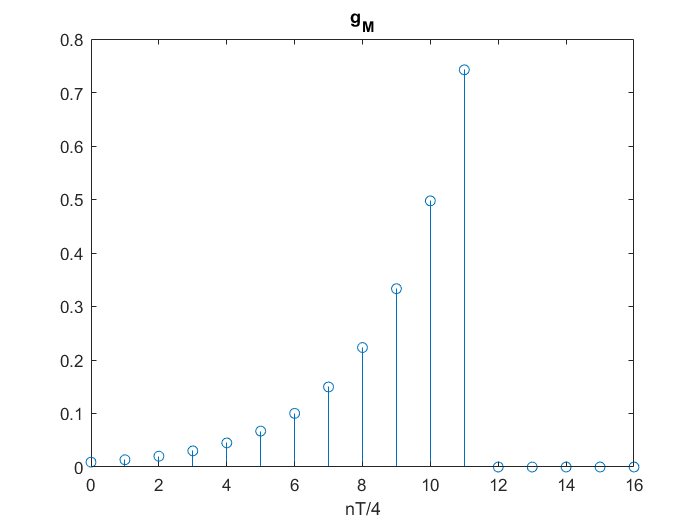
\includegraphics[width=\textwidth]{figs/A_gm.png} 
		\caption{Impulse response of the matched filter $g_{M}$ for the receiver in point A.}
		\label{fig:A_gm}
	\end{center}
\end{figure} 

The output of the matched filter is then sampled at $T$ starting from an initial offset called \emph{timing phase} $t_0$. In our case the choice of $t_0$ is made easy by the presence of the matched filter, as we can just choose the value $\bar{t}_0$, multiple of $T/4$, that is the index of the peak of the correlation between $q_c$ and $g_M$, then $t_0$ will be equal to $\bar{t}_0 T/4$. Following this reasoning we chose $\bar{t}_0=17$, equal also to the length of $g_M$ (see figure \ref{fig:A_gm}).

The signal is then passed to a linear equalizer (LE) derived by a particular case of a Decision Feedback Equalizer (DFE) where we only have the feedforward filter $c$ (see point B for the detailed analysis of the DFE). The signal at this point in the receiver system is called $x_k$ and is the result of the convolution of the input sequence $a_k$ with the overall impulse response $h_i = q_c * g_M$ that goes from $-N1$ to $N2$. We will call precursors the taps of $h$ that go from $-N1$ to $-1$ and postcursors the taps from $1$ to $N2$. To obtain the coefficients of $c$ we used the Wiener approach on the input random process and solved the Wiener-Hopf equation $\vt{c}_{opt}=\vt{R}^{-1}\vt{p}$ using the matrix $\vt{R}$ and vector $\vt{p}$ as in equations \ref{eq:wienerR} and \ref{eq:wienerp} with the parameter $M_2$ (the order of the feedback filter) set to $0$ because we have no feedback filter in this case. The free parameters that we have to choose are $M1$, the order of filter $c$ and $D$ the delay that it will introduce on the input sequence. We carried out this choice looking at the value of the cost function $J_{min}$ (see equation \ref{eq:jmin}) for each combination of the two parameters, preferring low values if possible to avoid increasing the complexity. The best choice in this case was $M1=5$ and $D=2$.
In figure \ref{fig:A_c} we plot the impulse response $c_i$ at sampling time $T$ as obtained from the Wiener solution. 

\begin{figure}[ht]
	\begin{center}   
		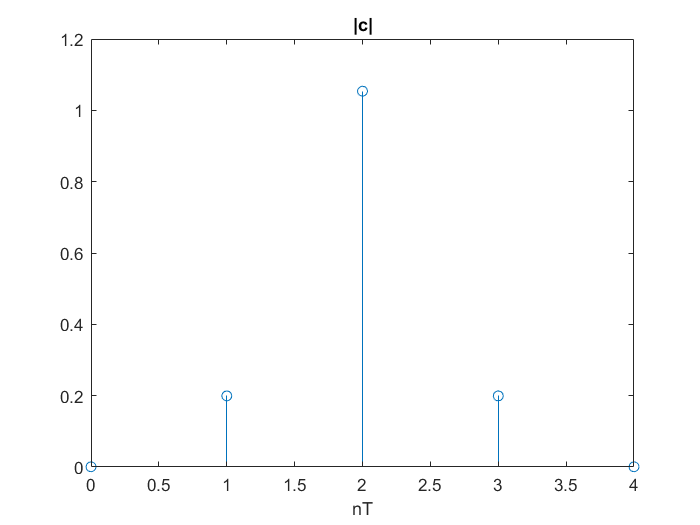
\includegraphics[width=\textwidth]{figs/A_c.png} 
		\caption{Magnitude of the impulse response of filter $c$ in point A.}
		\label{fig:A_c}
	\end{center}
\end{figure}

The aim of filtering with $c$ is to obtain an overall impulse response of the system that satisfies the Nyquist conditions for the absence of ISI at time $T$. This implies that in the ideal case $\psi=h*c$ is a delayed impulse centered on $D$ that is the delay. In our case the $\psi$ obtained is shown in figure \ref{fig:A_psi}. We can see the result is pretty good as all the precursors and postcursors are almost canceled by the equalizer. 


\begin{figure}[ht]
	\begin{center}   
		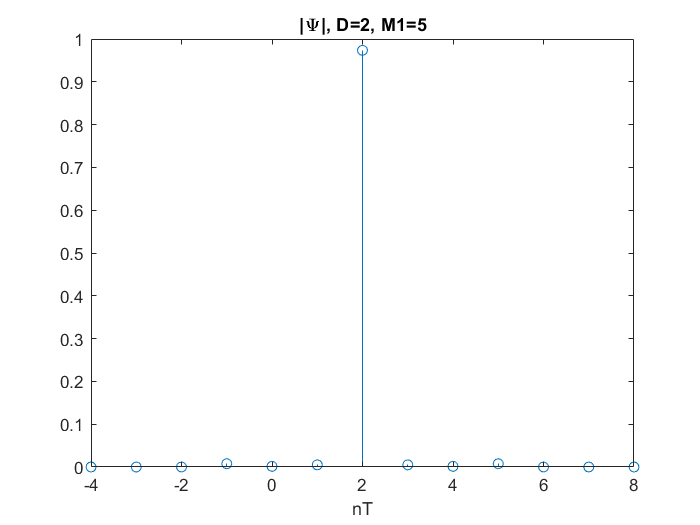
\includegraphics[width=\textwidth]{figs/A_psi.png} 
		\caption{Magnitude of the impulse response of the system $\psi$ in point A.}
		\label{fig:A_psi}
	\end{center}
\end{figure}

The detected symbols $a_{k-D}$ are chosen using a threshold detector that analyzes the sign of the imaginary and real part of the input complex value. Not that the same detector is also used at point B, C and D.


\section*{Point B}

For point B the system is the same as in point A up to the equalizer, so the choice of $\bar{t}_0=17$ is the same. The matched filter is the same as in point A, see figure \ref{fig:B_gm}. However in this case we equalize with a DFE, that is made of two filters called feedforward and feedback filter denoted by $c$ and $b$. The feedforward filter has the role of equalizing only the precursors of the overall impulse response, while the ISI due to postcursors will be canceled by filter $b$ positioned on a feedback loop between the output of the threshold detector and its input. 

\begin{figure}[ht]
	\begin{center}   
		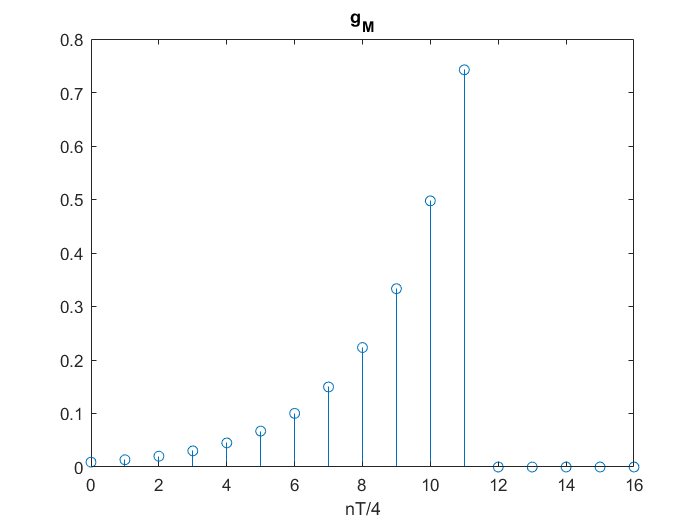
\includegraphics[width=\textwidth]{figs/B_gm.png} 
		\caption{Impulse response of the matched filter $g_{M}$ for the receiver in point B.}
		\label{fig:B_gm}
	\end{center}
\end{figure}

The computation of the optimal filters $c$ and $b$ is carried out using the Wiener filter approach. The relation between the input random process and the output is:
\begin{equation}
\begin{split}
y_k &= x_{FF,k} + x_{FB,k} \\
&= \sum_{i=0}^{M_1-1}c_ix_{k-i} + \sum_{j=1}^{M_2}b_ja_{k-D-j}
\end{split} 
\end{equation}
where $M1$ is the order of the feedforward filter, $M2$ is the order of the feedback filter and $a_{k-D}$ are the already detected past symbols fed back through $b$. Defining postcursors and precursors as in point A, we have that we can apply the Wiener-Hopf equations on the process:
\begin{equation}
y_k = \sum_{i=0}^{M_1-1}c_i \left(x_{k-i}-\sum_{j=1}^{M2}h_{j+D-i}a_{k-j-D} \right)
\end{equation}

The result can be easily computed as $c_{opt} = \vt{R}^{-1}\vt{p}$ once we find the atocorrelation matrix $\vt{R}$ and the correlation vector $\vt{p}$, expressed as \cite{nevio<3}:

\begin{equation} \label{eq:wienerR}
\mathbf{[R]}_{p,q} = \sigma_a^2 \left( \sum_{j=-N_1}^{N_2}h_jh^*_{j-(p-q)}-\sum_{j=1}^{M_2}h_{j+D-q}h^*_{j+d-p} \right) + r_{\tilde{w}}(p-q)
\end{equation}
\begin{equation} \label{eq:wienerp}
\mathbf{[p]}_p = \sigma_a^2 h^*_{D-p} \quad\quad\quad\quad\quad\quad p,q = 0,1,\dots,M_1-1
\end{equation}

where for a QPSK scheme $\sigma_a^2=2$ because it is the sum of two orthogonal components each with power $1$. The values of $r_{\tilde{w}}$ are the result of the autocorrelation of the noise after being filtered by $g_M$, so being the noise white we have $r_{\tilde{w}}(n)=N_0r_{g_M}(nT)$. At this point we can define the overall impulse response up to the threshold detector $\psi = h*c_{opt}$ and derive the optimal coefficients for filter $b$ as $b_i=-\psi_{i+D}$ for $i=1,\dots,M2$.

The value of the cost function $J_{min}$ obtained using these the optimal filters is :
\begin{equation} \label{eq:jmin}
J_{min} = \sigma^2_a \left( 1-\sum_{l=0}^{M_1-1} c_{opt,l}h_{D-l}\right)
\end{equation}

Again the parameters to choose are the order of filter $c$, $M1$, and the delay introduced $D$. This is because the order of $b$ can be chosen in such a way that all the postcursors are canceled by the feedback: $M2=N1+M1-D-1$, and also the expression of the autocorrelation matrix significantly simplifies. The choice is carried out by selecting the values that minimize the functional $J_{min}$, this time being $M1=5$ and $D=4$, and consequently $M2=2$ because $N1=2$. In figure \ref{fig:B_c}, \ref{fig:B_psi} and \ref{fig:B_b} we plot the resulting filters $c$, $\psi$ and $b$ at sampling time $T$. 

\begin{figure}[ht]
	\begin{center}   
		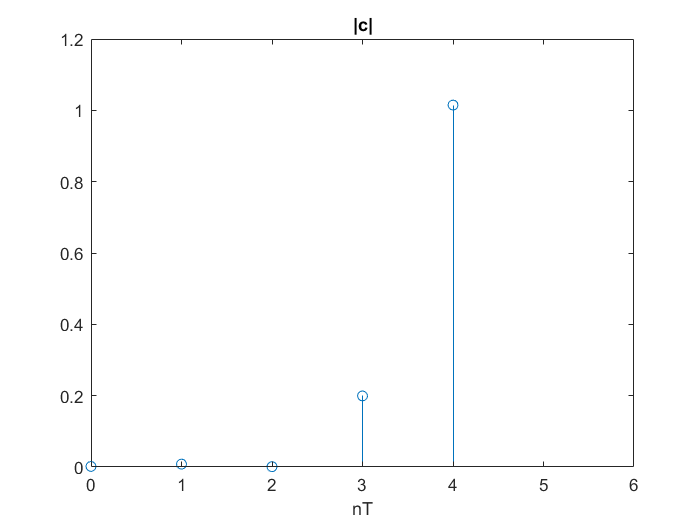
\includegraphics[width=\textwidth]{figs/B_c.png} 
		\caption{Magnitude of the impulse response of the filter $c$ (feedforward filter) for the receiver in point B.}
		\label{fig:B_c}
	\end{center}
\end{figure}

\begin{figure}[ht]
	\begin{center}   
		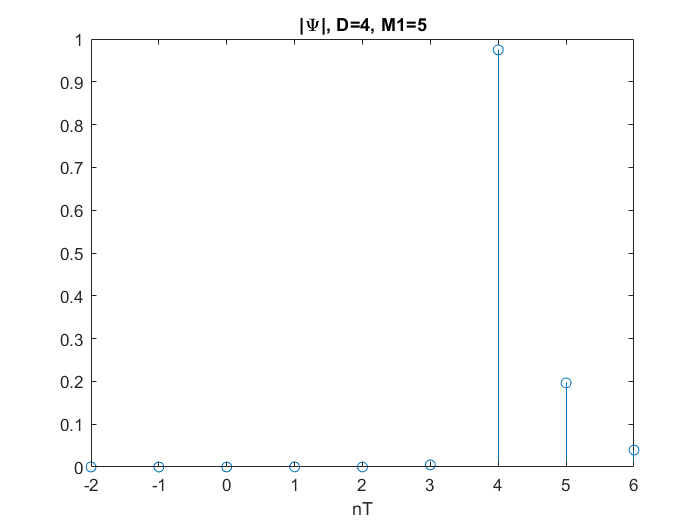
\includegraphics[width=\textwidth]{figs/B_psi.png} 
		\caption{Magnitude of the impulse response of the system $\psi$ in point B.}
		\label{fig:B_psi}
	\end{center}
\end{figure}

\begin{figure}[ht]
	\begin{center}   
		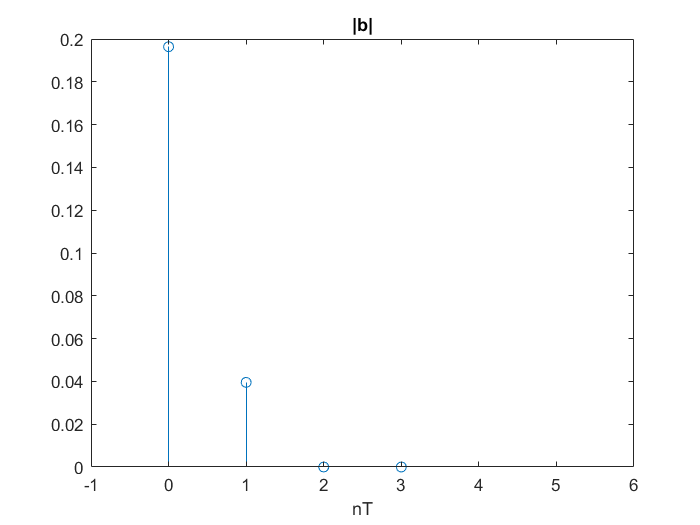
\includegraphics[width=\textwidth]{figs/B_b.png} 
		\caption{Magnitude of the impulse response of the filter $b$ (feedback filter) in point B.}
		\label{fig:B_b}
	\end{center}
\end{figure}

\section*{Point C}

\section*{Point D}

\section*{Point E}

\section*{Point F}

\section*{Simulation results}

\begin{figure}[ht]
	\begin{center}   
		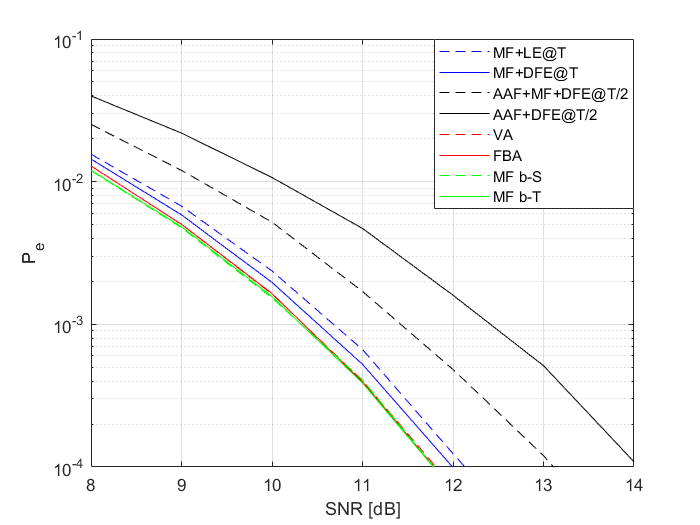
\includegraphics[width=\textwidth]{figs/SNR_Pe.png} 
		\caption{Results of the simulation over values of the SNR at the channel output from 8 dB to 14 dB.}
		\label{fig:B_b}
	\end{center}
\end{figure}


\begin{table}[htbp]
	\begin{center}
		\begin{tabular}{p{2.7cm}ccc}
			\toprule
			
			$nT_y$ & $h$ & $\hat{h}_{corr}$ & $\hat{h}_{ls}$\\
			\midrule
			0 & 1.0000  & 1.0054 & 0.9991  \\
			1 & 0.9635 & 0.9247 & 0.9613  \\
			2 & 0.4641 & 0.5002 & 0.5062 \\
			3 & -0.0001 & 0.0202 & 0.0255  \\
			4 & -0.2155 & -0.2549 & -0.2253\\
			\midrule
			%& \multicolumn{3}{c}{} \\
			& Real & Corr & LS \\
		    \cmidrule(lr){2-4}
		    $\sigma_w^2$ [dB] & -8 & -7.9776 & -8.0404  \\
			\bottomrule
		\end{tabular}
	\end{center}
	\label{tab:}
	\caption{.}
\end{table} 
 




\begin{thebibliography}{15}
	
	\bibitem{nevio<3}
	Nevio Benvenuto, Giovanni Cherubini,
	\textit{Algorithms for Communication Systems and their Applications}. 
	Wiley, 2002.
	

	
\end{thebibliography}

\end{document}